\documentclass{article}
\usepackage[utf8]{inputenc}
\usepackage[margin=0.8in]{geometry}
\usepackage{amsmath}
\usepackage{amssymb}
\usepackage{graphicx}
\usepackage{float}
\usepackage{hyperref}
\usepackage{xcolor}
\newcommand{\Do}{\partial}
\newcommand{\G}{\nabla}

\graphicspath{{images/}}

\title{Solutions to the Assignment - 3 : CS5480 - \\
Deep Learning}
\author{Vishwak Srinivasan\\
\texttt{CS15BTECH11043}}
\date{}

\begin{document}
\maketitle

\section*{Question 1}
\begin{flushleft}
The sample text used for this purpose is a 1565 character lyric of the song ``Speed of Sound'' by Coldplay. The lyrics were obtained from the website \href{https://songmeanings.com}{SongMeanings}.

There were 42 distinct characters.
\end{flushleft}

\section*{Question 2}
\subsection*{Part a}
\begin{flushleft}
Denote the hidden state at time \(t\) by \(h_{t}\), and the output by \(o_{t}\) and the input as \(x_{t}\). The notation for the weights will follow from the question. The question expects no biases, hence the equations will not contain them.
\begin{itemize}
\item [\textbf{i.}]
\begin{gather}
\text{Hidden Layer with activation: }h_{t} = \tanh(W_{xh}x_{t} + W_{hh}h_{t-1}) \\
\text{Output Layer without activation: }o_{t} = W_{ho}h_{t} \\
\text{Output Layer with activation: }\hat{y}_{t} = \mathrm{softmax}(o_{t})
\end{gather}

\item [\textbf{ii.}]
Denote the outer-product operator as \(\otimes\) and the Hadamard product as \(\odot\).

Since we are considering a cross-entropy loss (denoted by \(L\)), it is easy to see that the gradient with respect to the logits i.e., \(\hat{o}_{t}\), can be given by:
\begin{equation}
\left(\G_{o^{t}} L\right)_{i} = \frac{\Do L}{\Do L^{t}} \frac{\Do L^{t}}{\Do o_{i}^{t}} = \hat{y}_{i}^{t} - \mathbf{1}_{i = y^{t}}
\end{equation}
where \(\mathbf{1}_{p}\) denotes \(1\) if predicate \(p\) is satisfied and \(0\) otherwise.

Similarly, backpropping to the hidden state \(h_{t}\) gives us (using matrix calculus):
\begin{equation}
\label{hidden}
\G_{h^{t - 1}} L = \left(\frac{\Do h^{t}}{\Do h^{t - 1}}\right)^{T} (\G_{h^{t}} L) + \left(\frac{\Do o^{t - 1}}{\Do h^{t - 1}}\right)^{T} (\G_{o^{t - 1}} L) = W^{T} (\G_{h^{t}} L) \odot (1 - (h^{t})^{2}) + W_{ho}^{T} (\G_{o^{t - 1}} L)
\end{equation}

Now, say we go back to timestep \(k\) from timestep \(T\) backward. Due to this, by standard backprop through time, we get:
\begin{gather}
\displaystyle \G_{W_{ho}} L = \sum_{t=T}^{t=k} \sum_{i} \frac{\Do L}{\Do o_{i}^{t}} \G_{W_{ho}} o_{i}^{t} = \sum_{t=T}^{t=k} (\G_{o^{t}} L) (h^{t})^{T} = \sum_{t=T}^{t=k} (\G_{o^{t}} L) \otimes h^{t} \\
\label{hidden-full}
\displaystyle \G_{W_{hh}} L = \sum_{t=T}^{t=k} \sum_{i} \frac{\Do L}{\Do h_{i}^{t}} \G_{W_{hh}} h_{i}^{t} = (1 - (h^{t})^{2}) \odot \left((\G_{h^{t}} L) \otimes (h^{t-1})^{T}\right) \\
\displaystyle \G_{W_{xh}} L = \sum_{t=T}^{t=k} \sum_{i} \frac{\Do L}{\Do h_{i}^{t}} \G_{W_{xh}} h_{i}^{t} = (1 - (h^{t})^{2}) \odot \left((\G_{h^{t}} L) \otimes x^{t}\right)
\end{gather}

Some points:
\begin{itemize}
\item The terms \(1 - (h^{t})^{2}\) which occur in \ref{hidden}, \ref{hidden-full} are due to the \(\tanh\) non-linearity. The derivative of the \(\tanh\) function is \(1 - \tanh^{2}(z)\).
\end{itemize}

Now the weight update rule is simple:
\begin{gather}
\displaystyle W_{ho} := W_{ho} - \eta \G_{W_{ho}}L = W_{ho} - \eta \sum_{t=T}^{t=k} (\G_{o^{t}} L) \otimes h^{t} \\
\displaystyle W_{hh} := W_{ho} - \eta \G_{W_{hh}}L = W_{hh} - \eta \sum_{t=T}^{t=k} (1 - (h^{t})^{2}) \odot \left((\G_{h^{t}} L) \otimes (h^{t-1})^{T}\right) \\
\displaystyle W_{xh} := W_{xh} - \eta \G_{W_{xh}}L = W_{xh} - \eta \sum_{t=T}^{t=k} (1 - (h^{t})^{2}) \odot \left((\G_{h^{t}} L) \otimes x^{t}\right)
\end{gather}
\end{itemize}
\end{flushleft}

\subsection*{Part b}
\begin{flushleft}
\begin{itemize}
\item [\textbf{i.}] The network is trained using standard gradient descent, with a weight decay. To prevent exploding gradients, the gradients are clipped to have values between -2 and 2 only. The weight decay parameter is chosen to be \(10^{-4}\) and the learning rate is \(2\times 10^{-3}\). Below is the graph of training loss vs. number of epochs for 100 epochs. The sequence length taken was 50 (to get some comprehensible phrases). Number of hidden units is 250.

\begin{figure}[H]
\centering
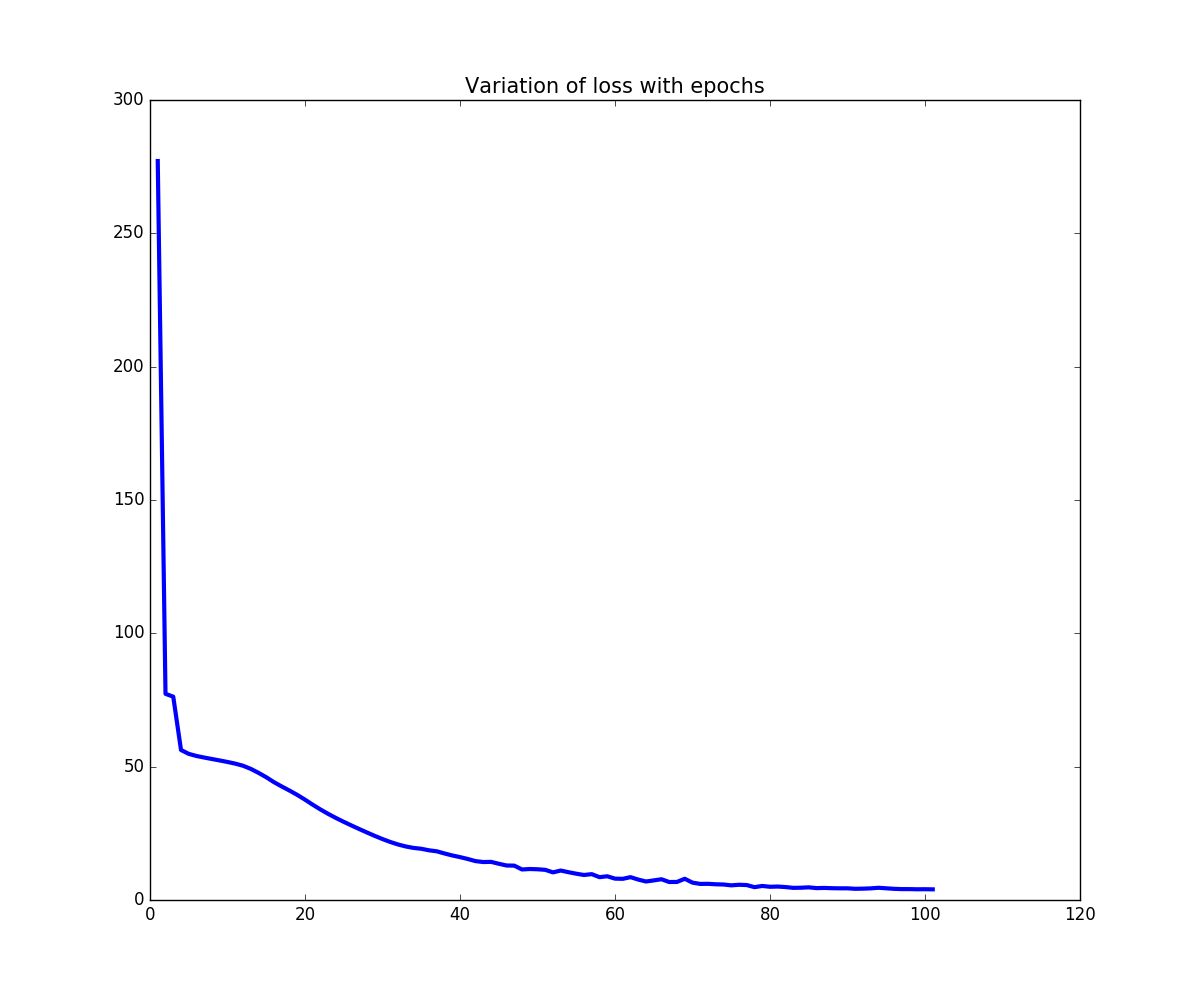
\includegraphics[width=0.75\linewidth]{RNN_training.png}
\end{figure}
\newpage
\item [\textbf{ii.}] For the same experiment as above, I generated 100 character sequences for every 20 epochs. Below are the generated texts:\\
\fbox{
\begin{minipage}{0.35\linewidth}
\textbf{At EPOCH 20:\\}
 then sound\\
re sou de then yound\\
re sou de then yound\\
re sou de then yound\\
re sou de then yound\\
re s
\end{minipage}
}
\fbox{
\begin{minipage}{0.45\linewidth}
\textbf{At EPOCH 40:\\}

Ifd be see le fhen you'd understand\\

If yound\\
Af shend\\
Af see it then you'd understand\\

If yound\\
Af
\end{minipage}
}
\fbox{
\begin{minipage}{0.9\linewidth}
\textbf{At EPOCH 60:\\}
All those sland\\
Ai dnee you desnde t ande you des it then you'd understand\\
Ah, when you see it then\\
\end{minipage}
}
\fbox{
\begin{minipage}{0.425\linewidth}
\textbf{At EPOCH 80:\\}
All those signs, I knew what they meant\\
Come things you can invent\\
And some get made, and aple gat\\
\end{minipage}
}
\fbox{
\begin{minipage}{0.425\linewidth}
\textbf{At EPOCH 100:\\}
All those signs, I knew what they meant\\
Aome things you can invent\\
And some get made, and all that\\
\end{minipage}
}
\item [\textbf{iii.}] At lower temperatures, this becomes a hard assignment, meaning this is equivalent to sampling that character whose probability is the highest. At higher temperatures, the logits become even, meaning that there will be random characters almost always.
Below are texts obtained with temperature 0.01:
\begin{figure}[H]
\begin{minipage}{0.3\textwidth}
\centering
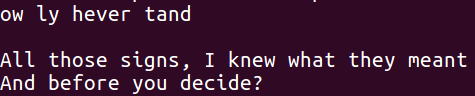
\includegraphics[width=0.95\textwidth]{100(1)-0_01.png}
\end{minipage}
\hfill
\begin{minipage}{0.3\textwidth}
\centering
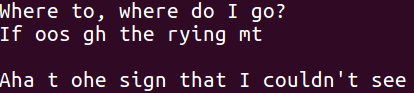
\includegraphics[width=0.95\textwidth]{100(2)-0_01.png}
\end{minipage}
\hfill
\begin{minipage}{0.3\textwidth}
\centering
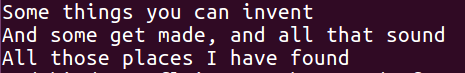
\includegraphics[width=0.95\textwidth]{100(3)-0_01.png}
\end{minipage}
\end{figure}
\begin{figure}[H]
\begin{minipage}{0.475\textwidth}
\centering
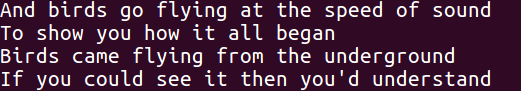
\includegraphics[width=0.95\textwidth]{100(4)-0_01.png}
\end{minipage}
\hfill
\begin{minipage}{0.475\textwidth}
\centering
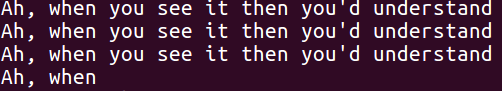
\includegraphics[width=0.95\textwidth]{100(5)-0_01.png}
\end{minipage}
\end{figure}

Below are texts obtained with temperature 2:
\begin{figure}[H]
\begin{minipage}{0.3\textwidth}
\centering
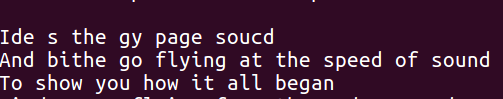
\includegraphics[width=0.95\textwidth]{100(1)-2.png}
\end{minipage}
\hfill
\begin{minipage}{0.3\textwidth}
\centering
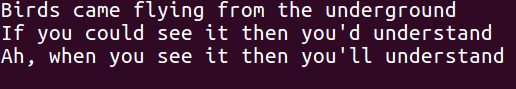
\includegraphics[width=0.95\textwidth]{100(2)-2.png}
\end{minipage}
\hfill
\begin{minipage}{0.3\textwidth}
\centering
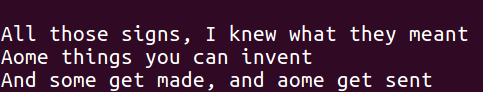
\includegraphics[width=0.95\textwidth]{100(3)-2.png}
\end{minipage}
\end{figure}
\begin{figure}[H]
\begin{minipage}{0.475\textwidth}
\centering
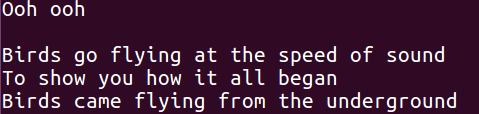
\includegraphics[width=0.95\textwidth]{100(4)-2.png}
\end{minipage}
\hfill
\begin{minipage}{0.475\textwidth}
\centering
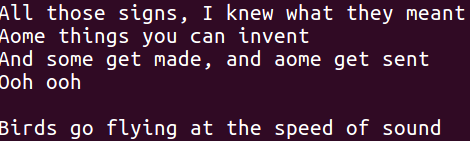
\includegraphics[width=0.95\textwidth]{100(5)-2.png}
\end{minipage}
\end{figure}

Below are the texts obtained with temperature 10. Note that each line corresponds to set different set of characters predicted.
\begin{figure}[H]
\centering
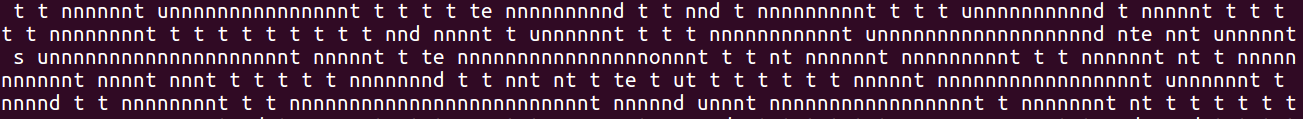
\includegraphics[width=0.75\linewidth]{500-10.png}
\end{figure}
\end{itemize}
\end{flushleft}

\subsection*{Part c}
\begin{flushleft}
\begin{itemize}
\item [\textbf{i.}]
Below is the training curve and sample text for double the number of hidden units taken earlier:
\begin{figure}[H]
\begin{minipage}{0.475\linewidth}
\centering
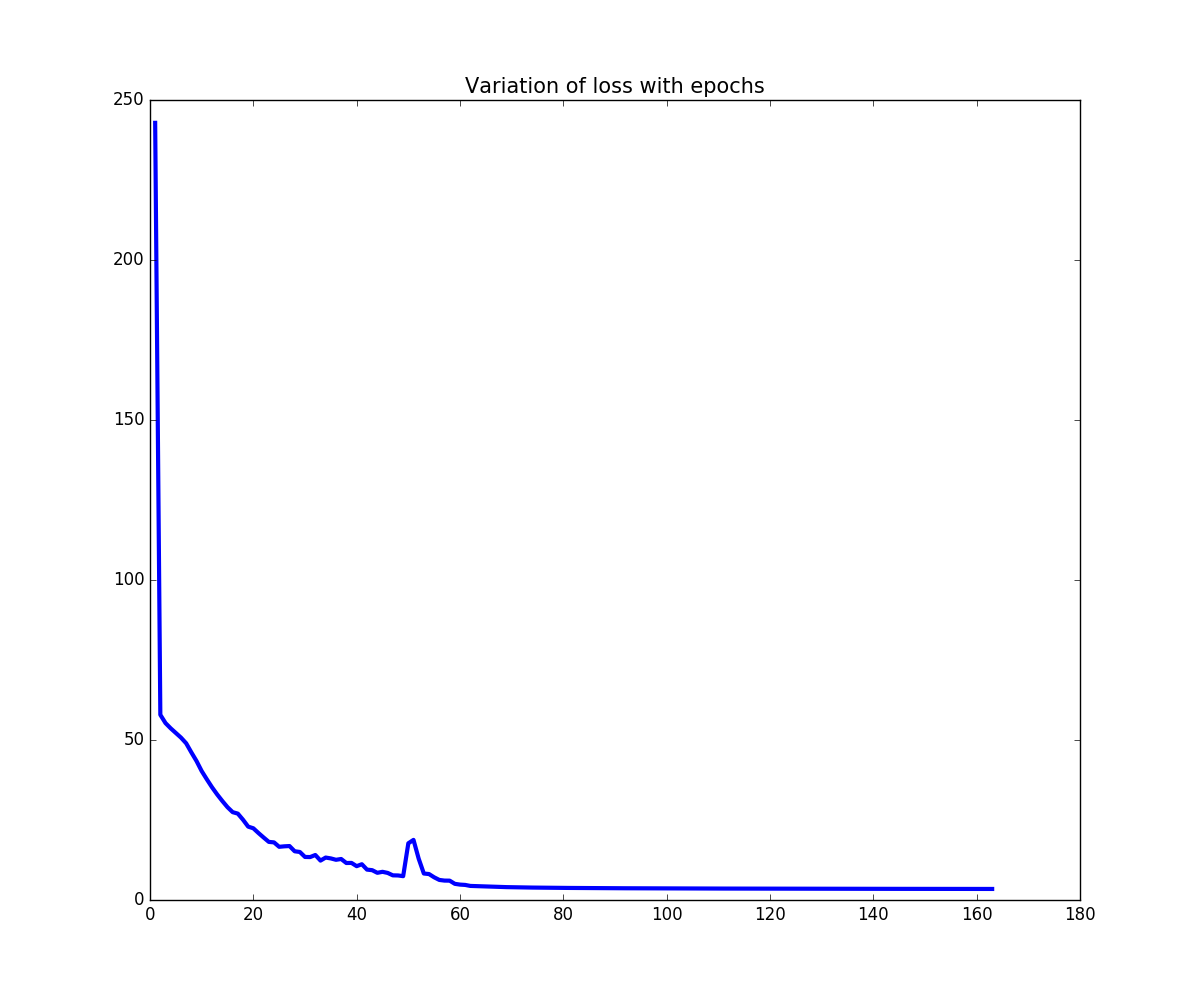
\includegraphics[width=0.9\textwidth]{RNN_training_HU2x.png}
\end{minipage}
\hfill
\begin{minipage}{0.475\linewidth}
\centering
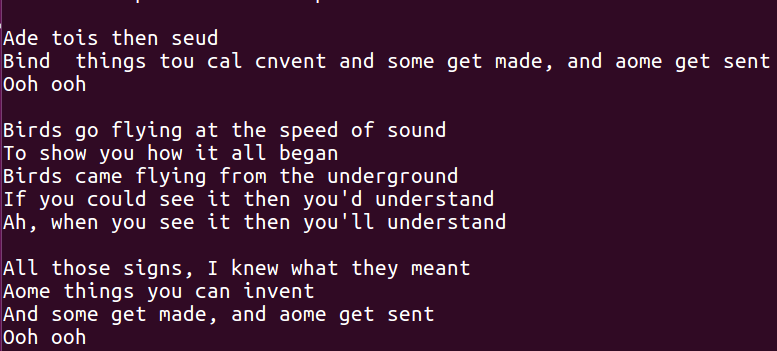
\includegraphics[width=0.9\textwidth]{RNN_text_HU2x.png}
\end{minipage}
\end{figure}

Below is the training curve and sample text for half the number of hidden units taken earlier:
\begin{figure}[H]
\begin{minipage}{0.475\linewidth}
\centering
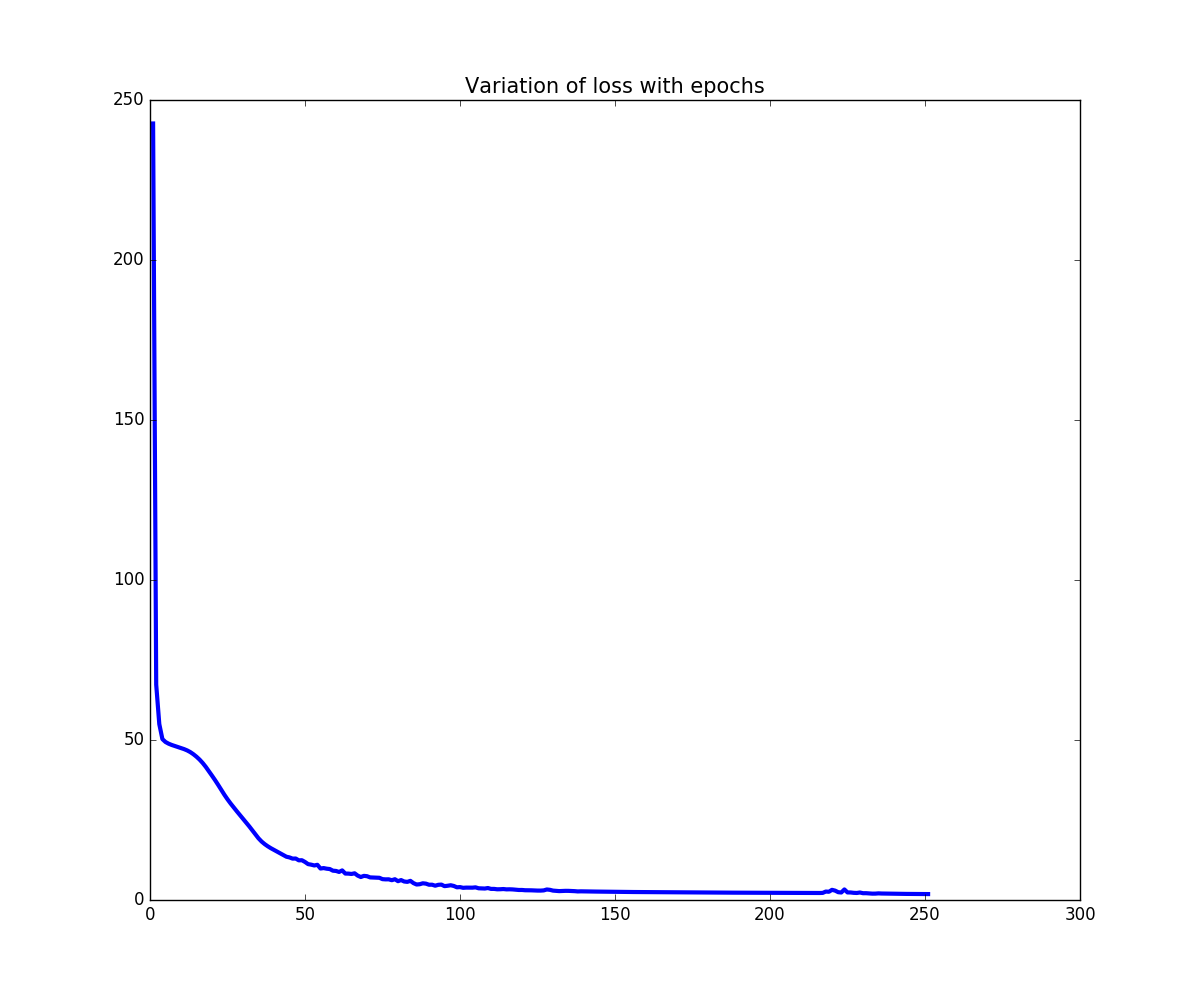
\includegraphics[width=0.9\textwidth]{RNN_training_HU0_5x.png}
\end{minipage}
\hfill
\begin{minipage}{0.475\linewidth}
\centering
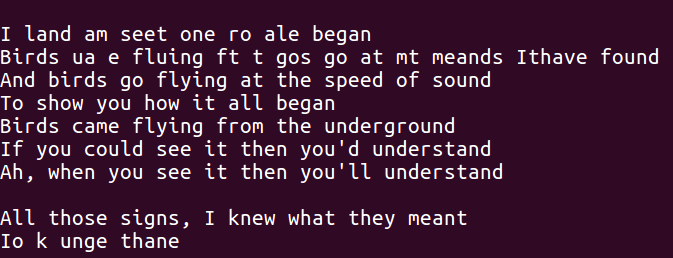
\includegraphics[width=0.9\textwidth]{RNN_text_HU0_5x.png}
\end{minipage}
\end{figure}

The enhancement in the text sampled from the RNN with higher hidden units could possibly be because of the enhanced capacity of the hidden layers. This could also mean that the RNN was capable of remembering pretty well. The same idea could be used for the RNN with lower hidden units but in the contrary i.e., the capacity is lesser, causing some gibberish.
\newpage
\item [\textbf{ii.}]
Below is the training curve and sample text for double the sequence length taken earlier:
\begin{figure}[H]
\begin{minipage}{0.475\linewidth}
\centering
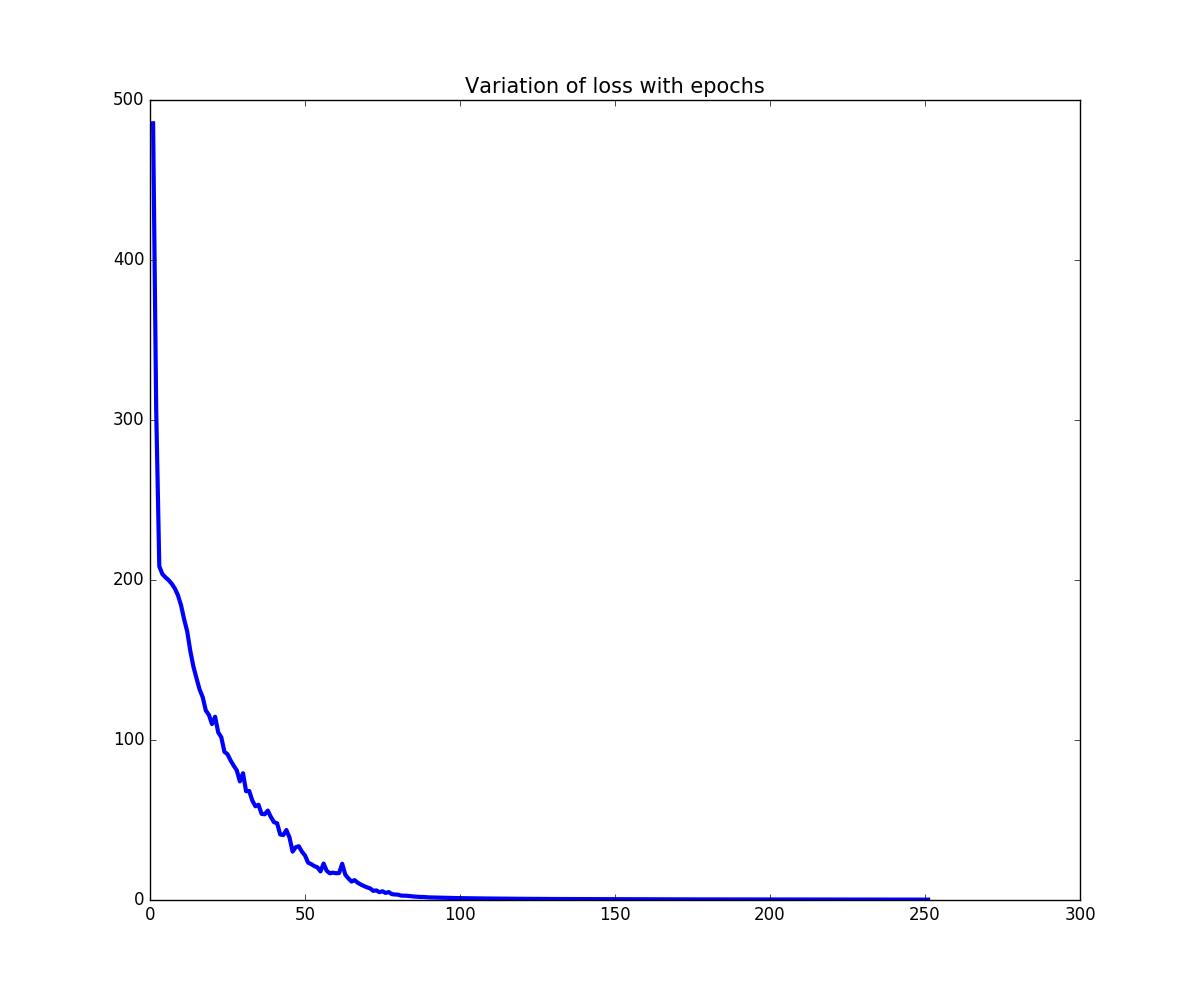
\includegraphics[width=0.9\textwidth]{RNN_training_SL2x.png}
\end{minipage}
\hfill
\begin{minipage}{0.475\linewidth}
\centering
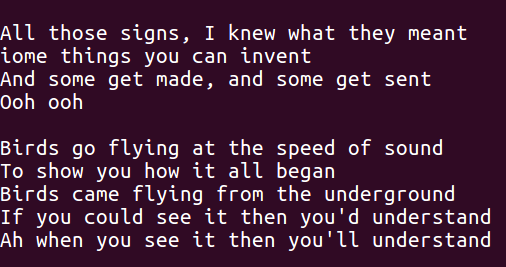
\includegraphics[width=0.9\textwidth]{RNN_text_SL2x.png}
\end{minipage}
\end{figure}

Below is the training curve and sample text for half the sequence length taken earlier:
\begin{figure}[H]
\begin{minipage}{0.475\linewidth}
\centering
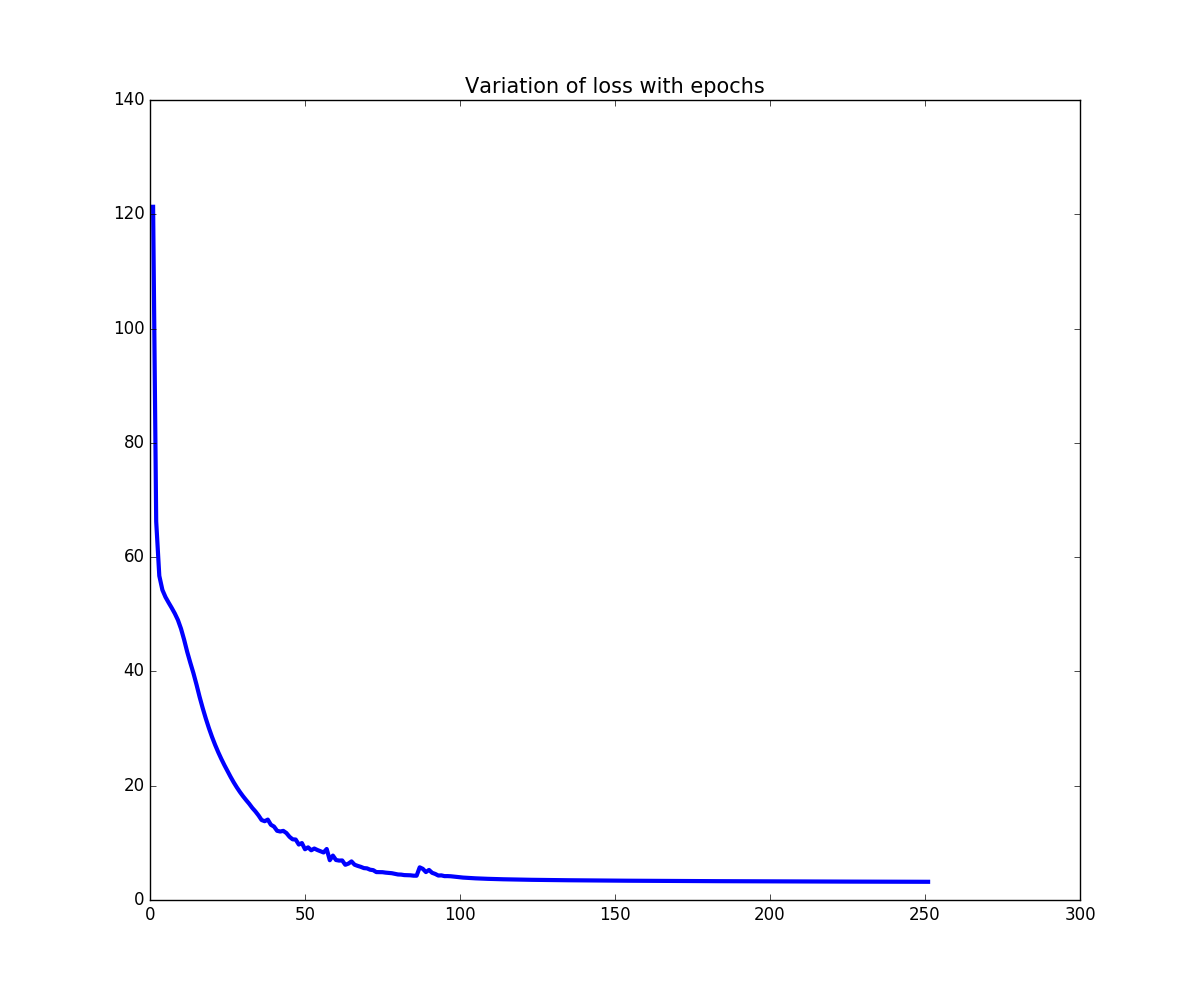
\includegraphics[width=0.9\textwidth]{RNN_training_SL0_5x.png}
\end{minipage}
\hfill
\begin{minipage}{0.475\linewidth}
\centering
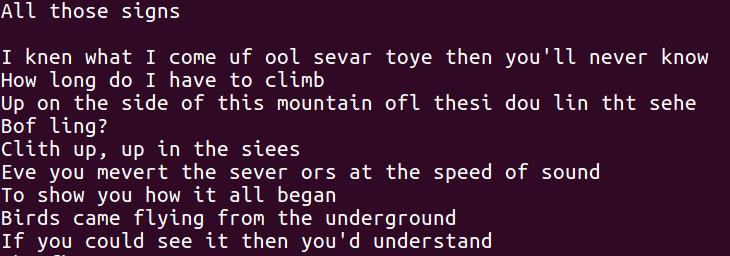
\includegraphics[width=0.9\textwidth]{RNN_text_SL0_5x.png}
\end{minipage}
\end{figure}
\end{itemize}

Increasing the sequence length, helps the RNN remember longer sequences effectively. This is why despite the same number of hidden units, the quality of the text sampled is good.
\end{flushleft}

\section*{Question 3}
\begin{flushleft}
My solution is based on this diagram:
\begin{figure}[H]
\centering
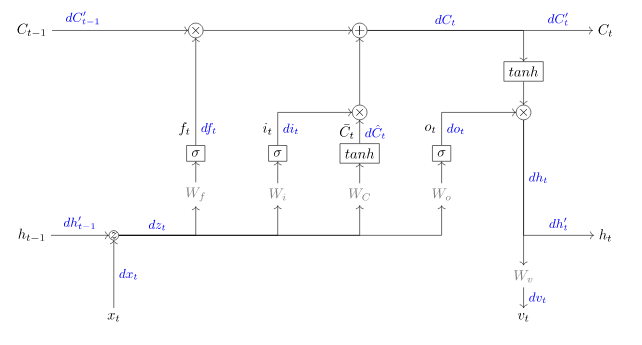
\includegraphics[width=0.5\linewidth]{lstm-map.png}
\end{figure}

The network is trained using standard gradient descent, with a weight decay. To prevent exploding gradients, the gradients are clipped to have values between -2 and 2 only. The weight decay parameter is chosen to be \(10^{-4}\) and the learning rate is 0.1. Number of hidden units is 100. Below is the training curve:
\begin{figure}[H]
\centering
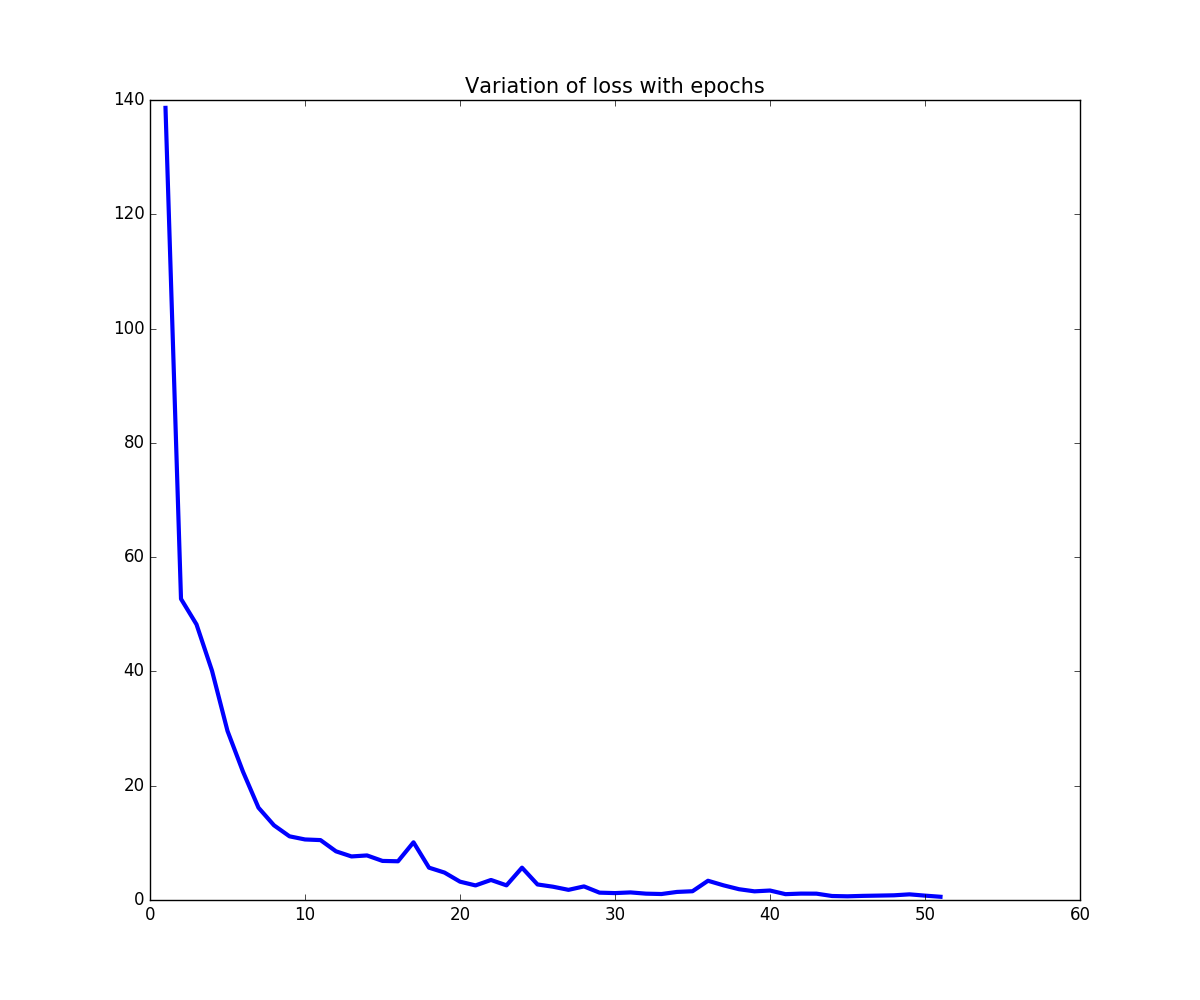
\includegraphics[width=0.75\linewidth]{LSTM_training.png}
\end{figure}

100 length text obtained after training for 50 epochs are shown below:
\begin{figure}[H]
\begin{minipage}{0.475\textwidth}
\centering
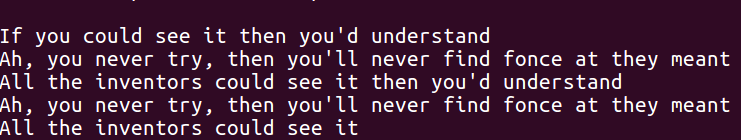
\includegraphics[width=0.9\textwidth]{LSTM_text1.png}
\end{minipage}
\hfill
\begin{minipage}{0.475\textwidth}
\centering
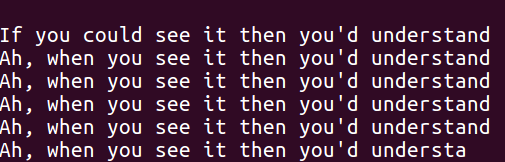
\includegraphics[width=0.9\textwidth]{LSTM_text2.png}
\end{minipage}
\end{figure}
\end{flushleft}
\end{document}
